
%(BEGIN_QUESTION)
% Copyright 2011, Tony R. Kuphaldt, released under the Creative Commons Attribution License (v 1.0)
% This means you may do almost anything with this work of mine, so long as you give me proper credit

Create a computer spreadsheet to calculate the reliability (in percent) as well as the Probability of Failure on Demand (PFD) for a single instrument with a given MTBF (in years) and a service time period (in days).  A sample layout is presented here, where yellow shading represents values to enter, and blue shading represents values calculated by the spreadsheet:

$$\includegraphics[width=15.5cm]{i03281x01.eps}$$

How will the reliability and PFD values compare for a whole {\it system} in which this single transmitter is an indispensible part?

\vskip 20pt \vbox{\hrule \hbox{\strut \vrule{} {\bf Suggestions for Socratic discussion} \vrule} \hrule}

\begin{itemize}
\item{} Explain how you may {\it test} your finished spreadsheet program to see that it correctly calculates reliability and PFD values. 
\end{itemize}

\underbar{file i03281}
%(END_QUESTION)





%(BEGIN_ANSWER)


%(END_ANSWER)





%(BEGIN_NOTES)


%INDEX% Computer spreadsheet exercise: instrument reliability and PFD
%INDEX% Safety, system reliability: Mean Time Between Failures (MTBF)
%INDEX% Safety, system reliability: percentage calculation
%INDEX% Safety, system reliability: probability of failure on demand (PFD)

%(END_NOTES)


